\subsection{Trigonometrische Funktionen}

\subsubsection{Amplitude ändern}
\underline{Strecken in y-Richtung:} \\
$f(x) = a\cdot sin(x)$ \\
$a < 1$: Stauchen \\
$a > 1$: Strecken

$f(x) = sin(x)$ in rot \\
$f(x) = 2\cdot sin(x)$ in grün \\
\scalebox{0.6}{
    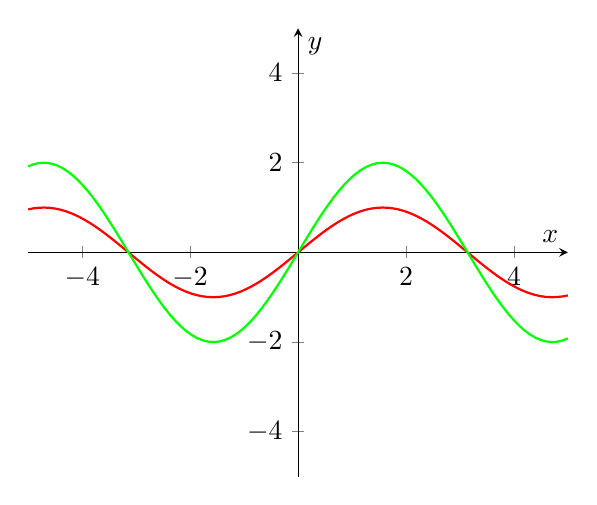
\begin{tikzpicture}
        \begin{axis}[
            axis lines=middle,
            xlabel={$x$},
            ylabel={$y$},
            %grid=major,
            domain=-5:5, % Range for x
            samples=100, % Number of samples for smoothness
            xmin=-5,xmax=5,ymin=-5,ymax=5
            ]
            \addplot[red, thick] {sin(deg(x))};
            \addplot[green, thick] {2*sin(deg(x))};
        \end{axis}
    \end{tikzpicture}
}

\subsubsection{Periode ändern}
\underline{Streckung in x-Richtung:} \\
$f(x) = a\cdot sin(b\cdot x)$ \\
$b < 1$: Stauchen \\
$b > 1$: Strecken

$f(x) = sin(x)$ in rot \\
$f(x) = sin(2\cdot x)$ in grün \\
\scalebox{0.6}{
    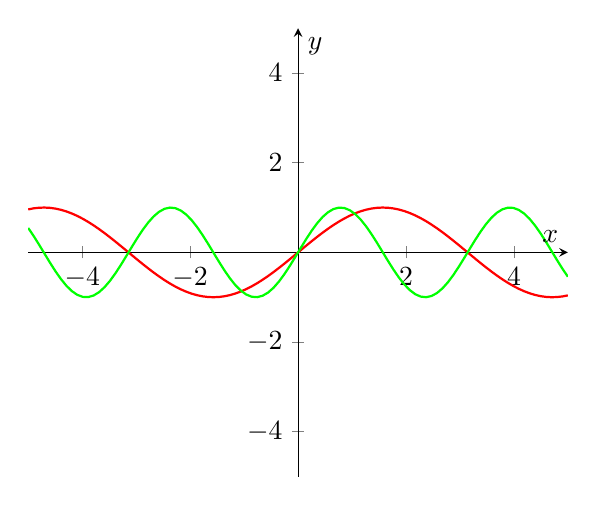
\begin{tikzpicture}
        \begin{axis}[
            axis lines=middle,
            xlabel={$x$},
            ylabel={$y$},
            %grid=major,
            domain=-5:5, % Range for x
            samples=100, % Number of samples for smoothness
            xmin=-5,xmax=5,ymin=-5,ymax=5
            ]
            \addplot[red, thick] {sin(deg(x))};
            \addplot[green, thick] {sin(deg(2*x))};
        \end{axis}
    \end{tikzpicture}
}

\subsubsection{Verschieben}
\underline{Verschieben in x-Richtung:} \\
$f(x) = a\cdot sin(b\cdot(x - c))$ \\
$c < 0$: Verschiebung nach links \\
$c > 0$: Verschiebung nach rechts \\
(beachte das minus wodurch das $c$ nochmal umgedreht wird und deshalb $c = 1$ zu $x - 1$ wird und nach rechts verschoben wird)

$f(x) = sin(x)$ in rot \\
$f(x) = sin(x-1)$ in grün \\
\scalebox{0.6}{
    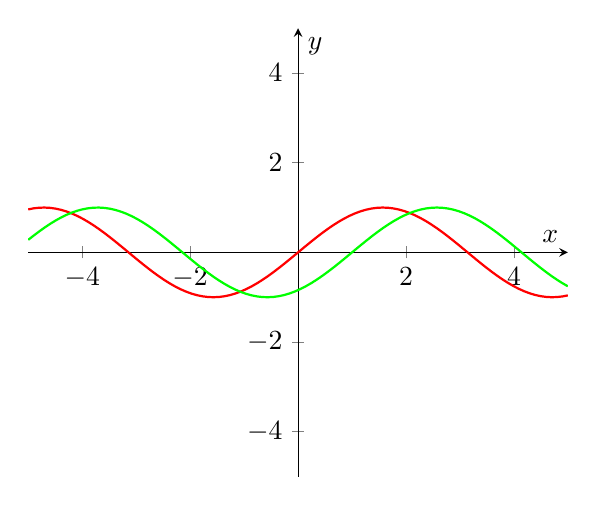
\begin{tikzpicture}
        \begin{axis}[
            axis lines=middle,
            xlabel={$x$},
            ylabel={$y$},
            %grid=major,
            domain=-5:5, % Range for x
            samples=100, % Number of samples for smoothness
            xmin=-5,xmax=5,ymin=-5,ymax=5
            ]
            \addplot[red, thick] {sin(deg(x))};
            \addplot[green, thick] {sin(deg(x-1))};
        \end{axis}
    \end{tikzpicture}
}

\underline{Verschieben in y-Richtung:} \\
$f(x) = a\cdot sin(b\cdot(x - c)) + d$ \\
$d < 0$: Verschiebung nach unten \\
$d > 0$: Verschiebung nach oben

$f(x) = sin(x)$ in rot \\
$f(x) = sin(x) - 1$ in grün \\
\scalebox{0.6}{
    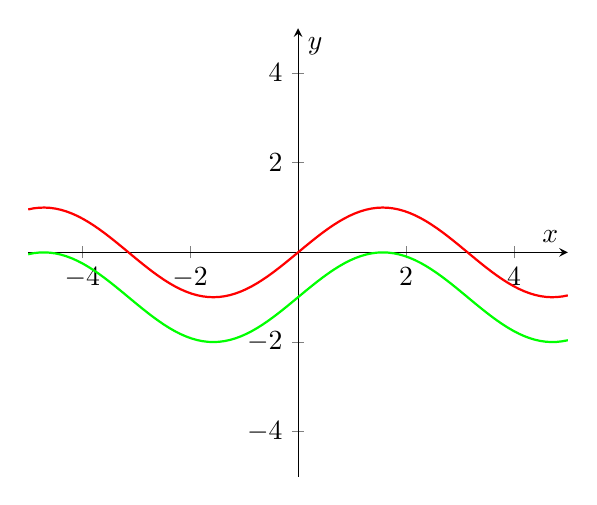
\begin{tikzpicture}
        \begin{axis}[
            axis lines=middle,
            xlabel={$x$},
            ylabel={$y$},
            %grid=major,
            domain=-5:5, % Range for x
            samples=100, % Number of samples for smoothness
            xmin=-5,xmax=5,ymin=-5,ymax=5
            ]
            \addplot[red, thick] {sin(deg(x))};
            \addplot[green, thick] {sin(deg(x)) - 1};
        \end{axis}
    \end{tikzpicture}
}
